\documentclass[12pt,a4paper]{article}
\usepackage{kotex}
\usepackage{graphicx}
\usepackage{hyperref}
\usepackage{indentfirst}
\usepackage{subcaption}
\usepackage{multirow}
\usepackage{flafter}
\usepackage{tikz}
\usetikzlibrary{arrows.meta, intersections, decorations.markings,
    positioning, backgrounds, through, calc, angles, quotes}
\setlength{\parskip}{2mm}
\usepackage{amsmath}
\usepackage[top=3cm, bottom=2.54cm, left=2.54cm, right=2.54cm]{geometry}
\usepackage[yyyymmdd]{datetime}
\renewcommand{\dateseparator}{-}
\usepackage{array}
\newcolumntype{L}[1]{>{
    \raggedright\let\newline\\\arraybackslash\hspace{0pt}}m{#1}}
\newcolumntype{C}[1]{>{
    \centering\let\newline\\\arraybackslash\hspace{0pt}}m{#1}}
\newcolumntype{R}[1]{>{
    \raggedleft\let\newline\\\arraybackslash\hspace{0pt}}m{#1}}

\begin{document}
\begin{titlepage}
    \centering
    \begin{tabular}{|C{15cm}|}
        \hline
        \rule{0in}{6ex}
        {\huge 물리학 및 실험 1\par} \\ 
        {\large 스마트 카트를 이용한 운동량 보존 법칙\par} \\
        \hline
    \end{tabular} \\
    \vspace{5cm}
    
\includegraphics[height=7.36cm]{logo.png}\par
    \vspace{3cm}
    \begin{tabular}{|l|l|l|l|l|l|}
        \hline
        과목 & \multicolumn{5}{l|}{물리학및실험1} \\
        \hline
        담당교수 & \multicolumn{2}{l|}{전계진} & 담당조교 &
            \multicolumn{2}{l|}{} \\
        \hline
        조 및 조원 &
        \multicolumn{5}{l|}{2조, 김민수 김민규 김민서 김백준 김연주} \\
        \hline
        제출일 & \multicolumn{5}{l|}{\today} \\
        \hline
        작성자 & 김민수 & 학번 & 20518009 & 학과 & 정보보호 \\
        \hline
    \end{tabular}
\end{titlepage}
\section{실험목적}
두 물체가 짧은 상호작용(탄성, 완전 비탄성, 폭발)하는 경우 상호작용 전후에 선운동량이
보존되는지 확인하여 운동량 보존법칙을 이해하고 상호작용 전후의 운동에너지가
보존되는지도 확인한다.
\section{서론}
\begin{itemize}
    \item 탄성 및 비탄성 충돌은 질량이 다른 두 개의 역학 카트로 수행된다.
        마그네틱 범퍼는 탄성 충돌에 사용되며, Velcro® 범퍼는 완전 비탄성 충돌에
        사용된다. 두 경우 모두 운동량은 보존된다.
    \item 카트 속도는 카트의 속도 센서로 기록된다. 카트의 마찰이 미치는 영향은 매우
        작다. 충돌 전후의 총 운동 에너지도 연구한다.
    \item 폭발, 탄성충돌, 완전 비탄성충돌을 스마트 카트를 이용하여 실험을 실시하고
        운동량 보존의 법칙을 확인하고 또한 에너지의 보존 여부를 확인한다.
\end{itemize}
\section{실험원리}
알짜 외력이 작용하지 않을 때 충돌하는 두 물체 전체 계의 총 운동량은 보존된다.
$$\textrm{충돌전의 운동량} = \textrm{충돌 후의 운동량}$$
$$m_A\vec{V}_A+m_B\vec{V}_B = m_A\vec{V}_{A}^{'} + m_B\vec{V}_{B}^{'}
\left[ \Sigma \vec{F}_{ext} = 0 \right]$$
두 개의 충돌하는 공으로 이루어진 계의 전체 운동량 벡터는 보존된다.

운동량 보존 법칙(law of conservation of momentum)의 일반적인 표현: 고립계의 전체
운동량은 일정하게 유지된다.

어떠한 충돌에서나 운동량은 보존 된다. 충돌에서 운동에너지도 보존되면 탄성충돌,
보존되지 않으면 비탄성 충돌이라 한다.

\begin{itemize}
    \item \begin{tabular}{l}
            탄성충돌: 운동량, 운동에너지 보존 \\
            \begin{tabular}{|c|}
                \hline
                $\textrm{충돌 전 전체 운동 에너지} =
                \textrm{충돌 후 전체 운동 에너지}$ \\
                $\frac{1}{2}m_AV_A^2 + \frac{1}{2}m_BV_B^2 =
                \frac{1}{2}m_AV_A^{'2} + \frac{1}{2}m_BV_B^{'2}$\\
                \hline
            \end{tabular}
        \end{tabular}
    \item 비탄성 충돌: 운동에너지 보존 안됨. 완전 비탄성 충돌은 한 덩어리가 되어
        같은 속도로 날아가는 것이다.
\end{itemize}
\section{실험기구 및 장치}
\begin{itemize}
    \item 역학트랙, 자기 범퍼, 벨크로 범퍼, 수준기
    \item 센서 실험장치: data 수집 및 분석 software (Capstone),
        스마트 카트 2대, 500g 추
\end{itemize}
\section{실험방법}
\begin{enumerate}
    \item [준비 1]
        \begin{enumerate}
            \item [1.] 역학 트랙을 설치하고 양쪽 끝에는 자기범퍼를 설치한다.
            \item [2.] Red 와 Blue의 두 Smart Cart에 자석 범퍼를 장착한다.
            \item [3.] 트랙위에 수준기를 올려놓고 좌우 수평을 맞춘다.
                어느 쪽으로도 살짝 움직였을 때 가속되지 않아야 한다.
            \item [4.] 두 카트의 질량과 사용할 500g 추의 질량을 정밀 측정한다.
                유효숫자는 4개로 한다.
        \end{enumerate}
    \item [준비 2]
        \begin{enumerate}
            \item [1.] 캡스톤을 실행한다.
            \item [2.] 스마트카트를 연결하고 내장된 센서 (위치, 속도)를 설정한다.
                (샘플링레이트는 50Hz로 맞춘다.)
            \item [3.] 표와 그래프 모드로 선택하여 표의 칼럼을 추가하여
                시간, 속도(Red), 속도(Blue), 그래프는 속도-시간 그래프에
                속도(Red), 속도(Blue)를 동일한 축에 나오도록 설정한다.
            \item [4.] 속도의 부호를 확인한다. 측정자의 입장에서 볼 때 두 수레의
                속도가 오른쪽으로 움직일 때 양수가 되도록 한다.
            \item [5.] 파란색 카트가 빨간색 카트의 오른쪽에 있는 상태에서
                마그네틱 범퍼가 모두 오른쪽에 있게 둔다.
                측정을 시작하고 두 카트를 오른쪽으로 민다. 두 속도 모두 양수여야
                한다. (카트를 움직여 확인해 본다. 카트는 카트의 마그네틱 범퍼
                방향으로 움직일 때 양의 속도로 인식한다.)
            \item [6.] 함수를 추가하고 그래프에 총운동량과 총운동에너지 그래프를
                각각 추가한다.
        \end{enumerate}
    \item [실험 1]
        \begin{enumerate}
            \item [A.] 
                \begin{enumerate}
                    \item [] 동일 질량 카트
                    \item [1.] 카트의 플런저를 눌러 2번 위치에 놓는다. 한 카트가
                        다른 카트와 접촉하고 있는 한 어느 플런저가 눌려 있는 것이
                        중요하지 않다. 트랙 중앙에서 두 개의 카트가 다른 카트와
                        접촉하도록 놓는다.
                    \item [2.] 빨간색 카트를 반대로 하고 있으므로 동일한 좌표계를
                        유지하려면 setup을 열고 빨간색 스마트 카트 위치 센서 옆에
                        있는 속성 버튼을 클릭하고 부호 변경을 선택한다.
                    \item [3.] 측정을 시작하고 카트가 움직이도록 트리거 누른다.
                        추 또는 매스바로 방아쇠를 누르는 것이 효과적이다.
                    \item [4.] 카트가 트랙 끝에 도달하기 전에 기록을 중지한다.
                    \item [5.] 속도 - 시간 그래프에서 도구를 사용하여 폭발 직후
                        빨간색 및 파란색 카트의 속도, 총 운동량, 총 운동에너지를
                        찾아서 표에 기록한다.
                \end{enumerate}
            \item [B.]
                \begin{enumerate}
                    \item [] 질량이 서로 다른 카트
                    \item [1.] 500g 추를 파란색 카트에 넣는다. Calculator의 $m_2$
                        값(추의 질량을 더한 값)을 변경한다. 파트 A의 1~4단계를
                        반복한다.
                \end{enumerate}
        \end{enumerate}
    \item [실험 2]
        \begin{enumerate}
            \item [A.] 
                \begin{enumerate}
                    \item [] 동일 질량 카트
                    \item [$\bullet$] 완전 비탄성 충돌을 위해 벨크로 범퍼를
                        이용한다.
                    \item [1.] Velcro® 범퍼가 서로 마주보게 하여 빨간색과 파란색
                        카트를 트랙에 정지해 놓는다. Calculator의 $m_2$ 값을
                        변경한다.
                    \item [2.] 빨간색 카트를 반대로 하고 있으므로 동일한 좌표계를
                        유지하려면 setup을 열고 빨간색 스마트 카트 위치 센서 옆에
                        있는 속성 버튼을 클릭하고 부호 변경을 선택한다.
                        (실험1과 동일)
                    \item [3.] 측정을 시작하고 빨간색 카트를 파란색 카트 쪽으로
                        밀어준다. 카트 중 하나가 트랙 끝에 도달하기 전에 측정을
                        중지한다.
                    \item [4.] 속도 대 시간 그래프에서 충돌 직전과 직후에 빨간
                        카트의 속도를 찾는다. 그래프를 확장하여 관심 있는 영역만
                        보는 것이 도움이 된다.
                    \item [5.] 파란색 수레의 초기 속도는 0이고 최종 속도는 빨간색
                    수레가 서로 붙어 있기 때문에 동일하다.
                \end{enumerate}
            \item [B.]
                \begin{enumerate}
                    \item [] 질량이 서로 다른 카트
                    \item [$\bullet$] 벨크로 범퍼를 이용한다.
                    \item [1.] 500g 추를 파란색 카트에 넣는다.
                    Calculator의 $m_2$ 값을 변경한다. 파트 A의 1~4단계를 반복한다.
                \end{enumerate}
        \end{enumerate}
    \item [실험 3]
        \begin{enumerate}
            \item [A.] 
                \begin{enumerate}
                    \item [] 동일 질량 카트
                    \item [$\bullet$] 탄성 충돌을 위해 자기 범퍼를 이용한다.
                    \item [1.] 마그네틱 범퍼가 서로 마주보게 하여 빨간색과 파란색
                        카트를 트랙에 정지해 놓는다. 이제 빨간색 카트는 원래 양의
                        방향에 있고 파란색 카트는 반전되었으므로 데이터 요약을 열고
                        빨간색 스마트 카트 위치 센서 옆에 있는 속성 버튼을 클릭하고
                        기호 변경을 선택 취소하고 파란색 스마트 카트 위치 센서
                        속성을 열고 기호 변경 선택한다
                    \item [2.] 마그네틱 범퍼가 서로 마주보게 하여 빨간색 및 파란색
                        카트를 트랙에 정지해 놓는다. Calculator의 $m_2$ 값을
                        변경한다.
                    \item [3.] 측정을 시작하고 빨간색 카트를 파란색 카트 쪽으로
                        밀어준다.
                    \item [4.] 카트 중 하나가 트랙 끝에 도달하기 전에 측정을
                        중지한다.
                    \item [5.] 속도 대 시간 그래프에서 충돌 직전과 직후에 빨간
                        카트의 속도를 찾는다. 총 운동량, 총 운동에너지도 찾아서
                        표에 기록한다. 그래프를 확장하여 관심 있는 영역만 보는 것이
                        도움이 된다.
                    \item [6.] 파란색 수레의 초기 속도는 0이다. 파란색 카트의 최종
                        속도를 찾는다.
                \end{enumerate}
            \item [B.]
                \begin{enumerate}
                    \item [] 질량이 서로 다른 카트
                    \item [$\bullet$] 탄성 충돌을 위해 자기 범퍼를 이용한다.
                    \item [1.] 500g 추를 파란색 카트에 넣는다. Calculator의
                    $m_2$ 값을 변경한다. 파트 A의 1~6단계를 반복한다.
                \end{enumerate}
        \end{enumerate}
\end{enumerate}
\section{실험 결과 및 분석}
빨간 카트의 질량: 0.270kg

파란 카트의 질량: 0.270kg

추의 질량: 0.5kg
\begin{figure}[!h]
    \centering
    \resizebox{15.6cm}{!}{
    \begin{tabular}{|c|c|c|c|c|c|c|c|}
        \hline
        & 카트 질량 & \begin{tabular}{c}
            $m_r$ \\
            $[kg]$
        \end{tabular} & \begin{tabular}{c}
            $m_b$ \\
            $[kg]$
        \end{tabular} & \begin{tabular}{c}
            $V_{r, init}$ \\
            $[m/s]$
        \end{tabular} & \begin{tabular}{c}
            $V_{b, init}$ \\
            $[m/s]$
        \end{tabular} & \begin{tabular}{c}
            $V_{r, fin}$ \\
            $[m/s]$
        \end{tabular} & \begin{tabular}{c}
            $V_{b, fin}$ \\
            $[m/s]$
        \end{tabular} \\
        \hline
        \multirow{2}{*}{폭발} & 동일 질량 & 0.270 & 0.270 & 0.0 & 0.0 & -0.567 &
            0.573 \\
        \cline{2-8}
        & 다른 질량 & 0.270 & 0.770 & 0.0 & 0.0 & -0.681 & 0.247 \\
        \cline{2-8}
        \hline
        \multirow{2}{*}{완전 비탄성 출돌} & 동일 질량 & 0.270 & 0.270 & 0.505 &
            0.0 & 0.251 & 0.251 \\
        \cline{2-8}
        & 다른 질량 & 0.270 & 0.770 & 0.480 & 0.0 & 0.125 & 0.125 \\
        \cline{2-8}
        \hline
        \multirow{2}{*}{탄성 충돌} & 동일 질량 & 0.270 & 0.270 & 0.374 & 0.0 &
            0.0 & 0.366 \\
        \cline{2-8}
        & 다른 질량 & 0.270 & 0.770 & 0.466 & 0.0 & -0.197 & 0.233 \\
        \hline
    \end{tabular}
    }
    \caption{\label{table1}}
\end{figure}
\begin{figure}[!h]
    \centering
    \begin{subfigure}[]{0.4\textwidth}
        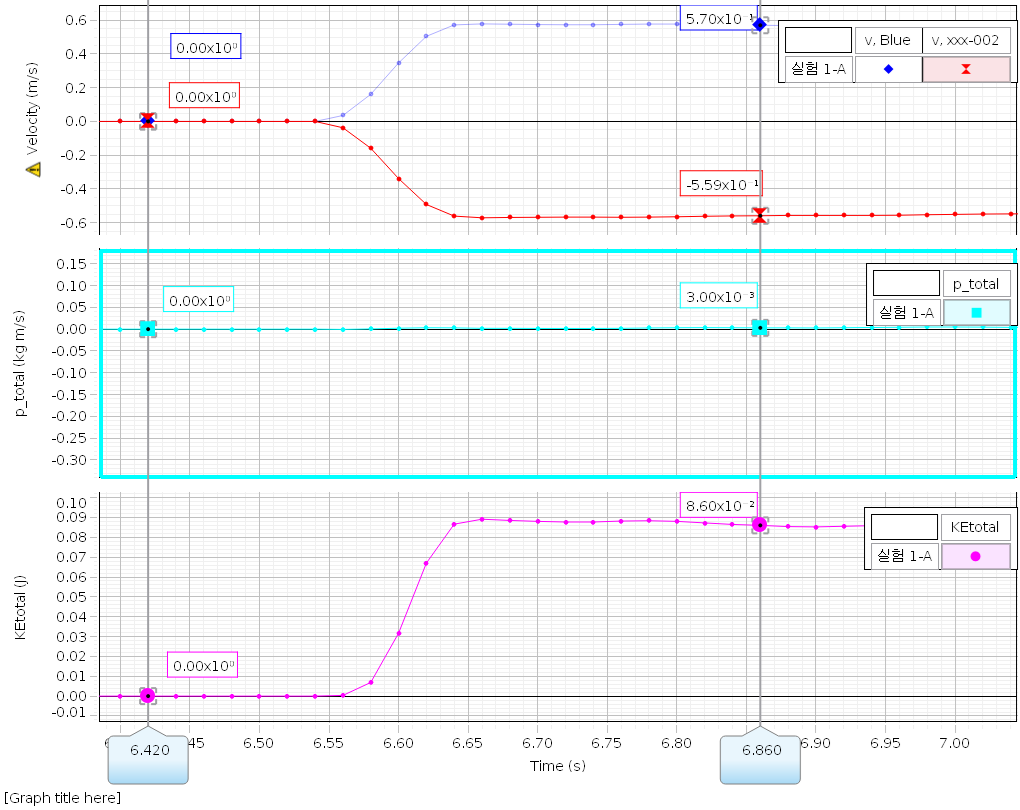
\includegraphics[height=4.36cm]{W10_1-A.png}
        \caption{\label{fig1-A}동일 질량}
    \end{subfigure}
    \begin{subfigure}[]{0.4\textwidth}
        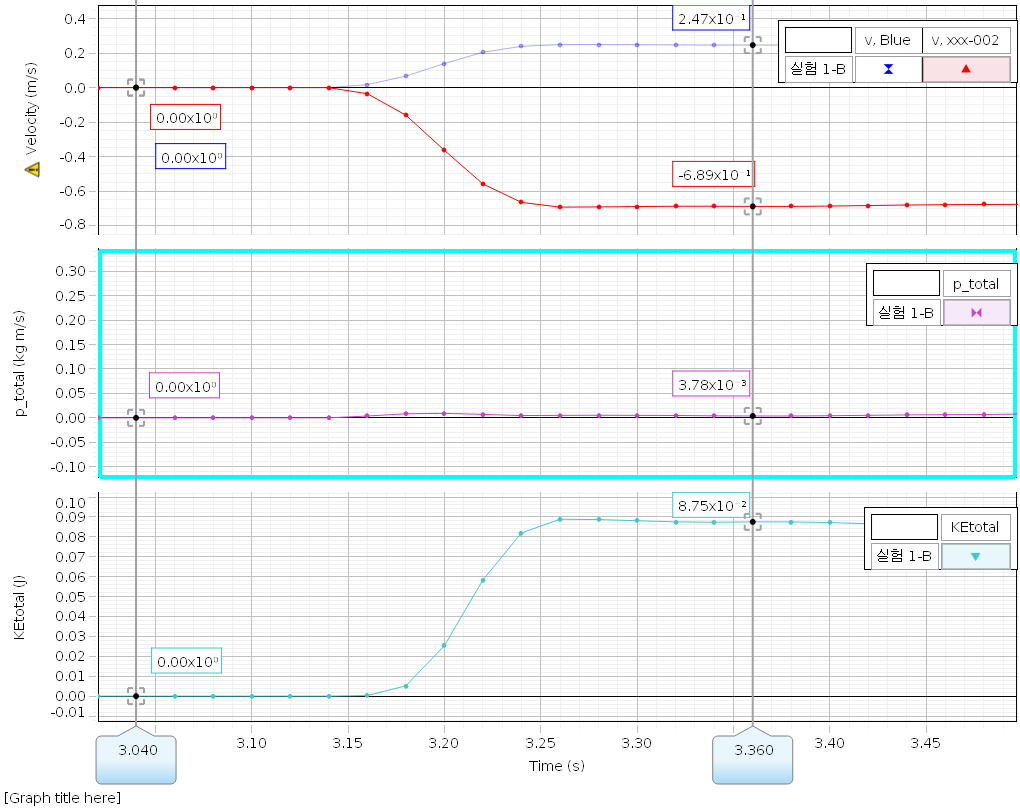
\includegraphics[height=4.36cm]{W10_1-B.png}
        \caption{\label{fig1-B}다른 질량}
    \end{subfigure}
    \caption{\label{fig1}폭발}
\end{figure}
\begin{figure}[!h]
    \centering
    \begin{subfigure}[]{0.4\textwidth}
        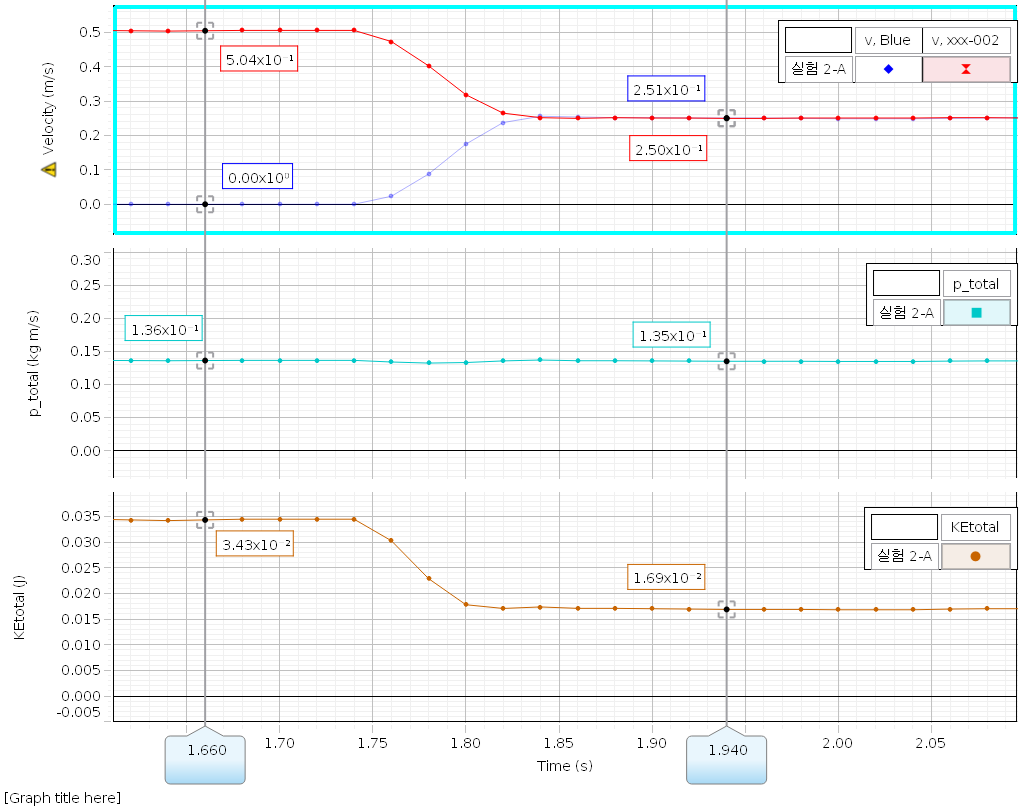
\includegraphics[height=4.36cm]{W10_2-A.png}
        \caption{\label{fig2-A}동일 질량}
    \end{subfigure}
    \begin{subfigure}[]{0.4\textwidth}
        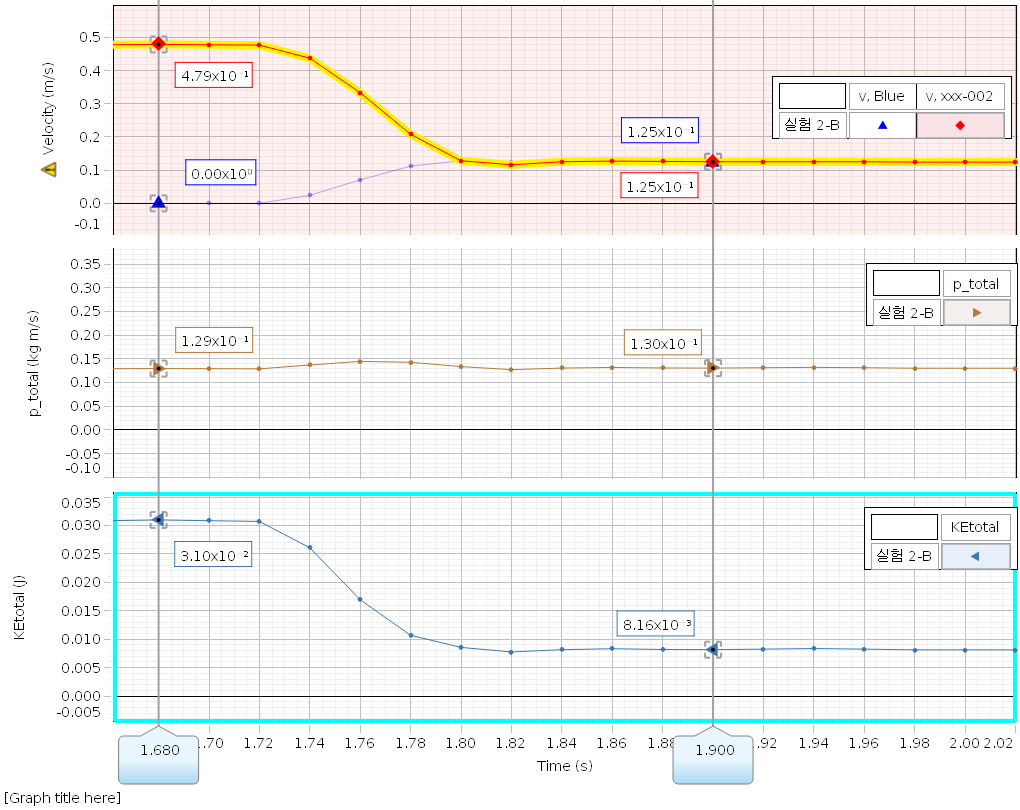
\includegraphics[height=4.36cm]{W10_2-B.png}
        \caption{\label{fig2-B}다른 질량}
    \end{subfigure}
    \caption{\label{fig2}완전 비탄성 충돌}
\end{figure}
\begin{figure}[!h]
    \centering
    \begin{subfigure}[]{0.4\textwidth}
        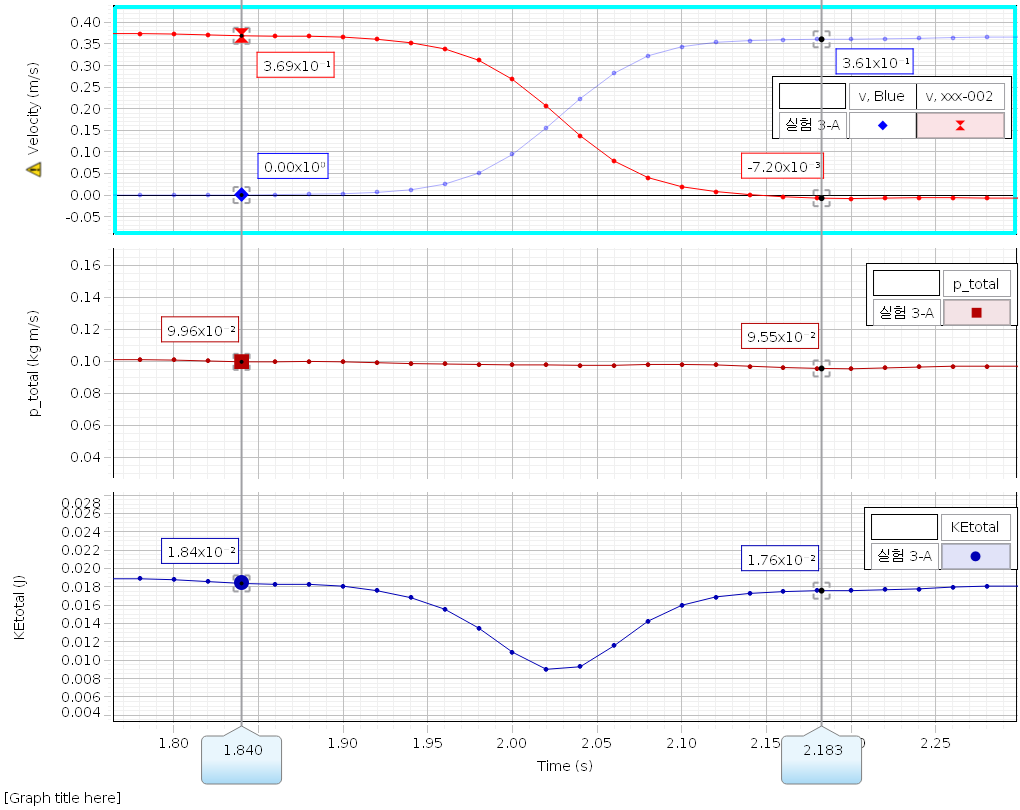
\includegraphics[height=4.36cm]{W10_3-A.png}
        \caption{\label{fig3-A}동일 질량}
    \end{subfigure}
    \begin{subfigure}[]{0.4\textwidth}
        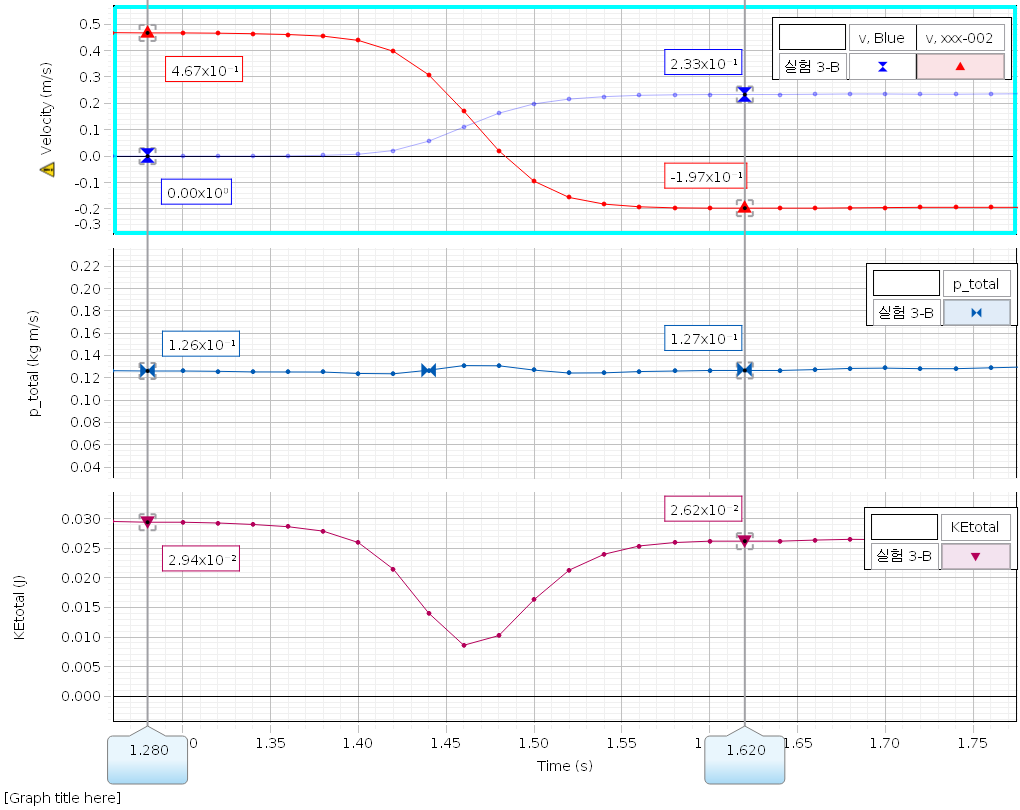
\includegraphics[height=4.36cm]{W10_3-B.png}
        \caption{\label{fig3-B}다른 질량}
    \end{subfigure}
    \caption{\label{fig3}탄성 충돌}
\end{figure}
\begin{figure}[!h]
    \centering
    \resizebox{15.6cm}{!}{
    \begin{tabular}{|c|c|c|c|c|c|c|c|}
        \hline
        & 카트 질량 & \begin{tabular}{c}
            $P_{r,init}$ \\
            $[kg \cdot m/s]$
        \end{tabular} & \begin{tabular}{c}
            $P_{b,init}$ \\
            $[kg \cdot m/s]$
        \end{tabular} & \begin{tabular}{c}
            $P_{total,init}$ \\
            $[kg \cdot m/s]$
        \end{tabular} & \begin{tabular}{c}
            $P_{r,fin}$ \\
            $[kg \cdot m/s]$
        \end{tabular} & \begin{tabular}{c}
            $P_{b,fin}$ \\
            $[kg \cdot m/s]$
        \end{tabular} & \begin{tabular}{c}
            $P_{total,fin}$ \\
            $[kg \cdot m/s]$
        \end{tabular} \\
        \hline
        \multirow{2}{*}{폭발} & 동일 질량 & 0.0 & 0.0 & 0.0 & -0.153 & 0.155 &
            0.00164 \\
        \cline{2-8}
        & 다른 질량 & 0.0 & 0.0 & 0.0 & -0.186 & 0.190 & 0.00433 \\
        \cline{2-8}
        \hline
        \multirow{2}{*}{완전 비탄성 출돌} & 동일 질량 & 0.136 & 0.0 & 0.136 &
            0.0677 & 0.0679 & 0.136 \\
        \cline{2-8}
        & 다른 질량 & 0.129 & 0.0 & 0.129 & 0.0338 & 0.0965 & 0.130 \\
        \cline{2-8}
        \hline
        \multirow{2}{*}{탄성 충돌} & 동일 질량 & 0.0993 & 0.0 & 0.0996 & -0.00109
        & 0.0971 & 0.0960 \\
        \cline{2-8}
        & 다른 질량 & 0.126 & 0.0 & 0.126 & -0.0532 & 0.0180 & 0.127 \\
        \hline
    \end{tabular}
    }
    \caption{\label{table2}}
\end{figure}
\begin{figure}[!h]
    \centering
    \resizebox{15.6cm}{!}{
    \begin{tabular}{|c|c|c|c|c|c|c|c|c|}
        \hline
        & 카트 질량 & \begin{tabular}{c}
            $K\!E_{r,init}$ \\
            $[J]$
        \end{tabular} & \begin{tabular}{c}
            $K\!E_{b,init}$ \\
            $[J]$
        \end{tabular} & \begin{tabular}{c}
            $K\!E_{total,init}$ \\
            $[J]$
        \end{tabular} & \begin{tabular}{c}
            $K\!E_{r,fin}$ \\
            $[J]$
        \end{tabular} & \begin{tabular}{c}
            $K\!E_{b,fin}$ \\
            $[J]$
        \end{tabular} & \begin{tabular}{c}
            $K\!E_{total,fin}$ \\
            $[J]$
        \end{tabular} & \begin{tabular}{c}
            $\Delta K\!E_{total}$ \\
            $[J]$
        \end{tabular}\\
        \hline
        \multirow{2}{*}{폭발} & 동일 질량 & 0.0 & 0.0 & 0.0 & 0.0435 & 0.0446 &
            0.0882 & 0.0882 \\
        \cline{2-9}
        & 다른 질량 & 0.0 & 0.0 & 0.0 & 0.0639 & 0.0234 & 0.0873 & 0.0873 \\
        \cline{2-9}
        \hline
        \multirow{2}{*}{완전 비탄성 출돌} & 동일 질량 & 0.0345 & 0.0 & 0.0345 &
            0.00841 & 0.00848 & 0.0169 & -0.0176 \\
        \cline{2-9}
        & 다른 질량 & 0.0310 & 0.0 & 0.0310 & 0.00219 & 0.00614 & 0.00833 &
            -0.02267 \\
        \cline{2-9}
        \hline
        \multirow{2}{*}{탄성 충돌} & 동일 질량 & 0.0183 & 0.0 & 0.0183 & 0.0 &
            0.0176 & 0.0176 & -0.0007 \\
        \cline{2-9}
        & 다른 질량 & 0.0290 & 0.0 & 0.0290 & 0.00524 & 0.0210 & 0.0262 &
            -0.0028 \\
        \hline
    \end{tabular}
    }
    \caption{\label{table3}}
\end{figure}
\begin{figure}[!h]
    \centering
    \begin{subfigure}[]{0.3\textwidth}
        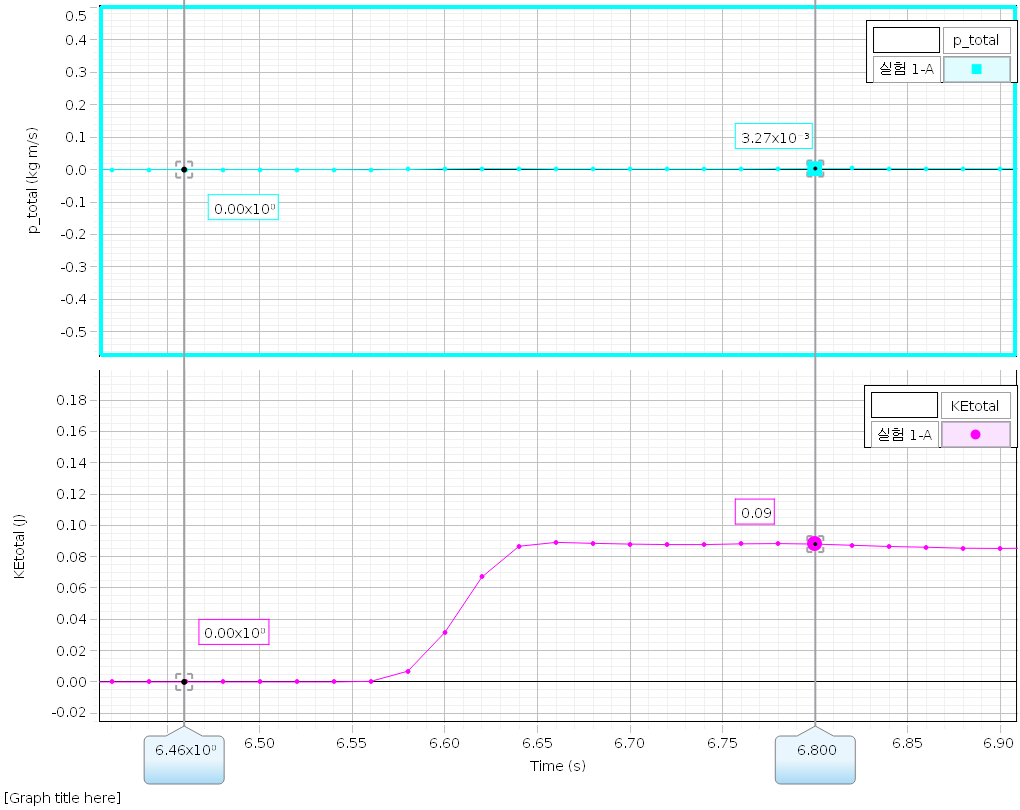
\includegraphics[height=4.36cm]{W10_exp.png}
        \caption{\label{fig4-A}폭발}
    \end{subfigure}
    \begin{subfigure}[]{0.3\textwidth}
        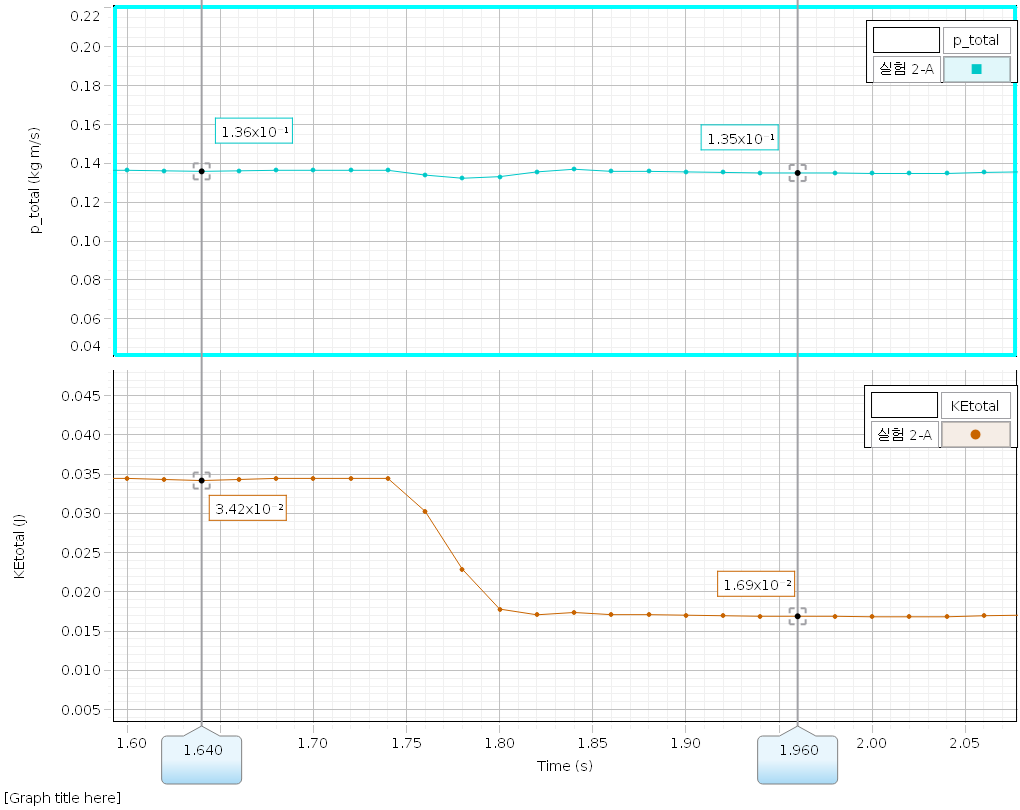
\includegraphics[height=4.36cm]{W10_tnelastic.png}
        \caption{\label{fig4-B}완전 비탄성 충돌}
    \end{subfigure}
    \begin{subfigure}[]{0.3\textwidth}
        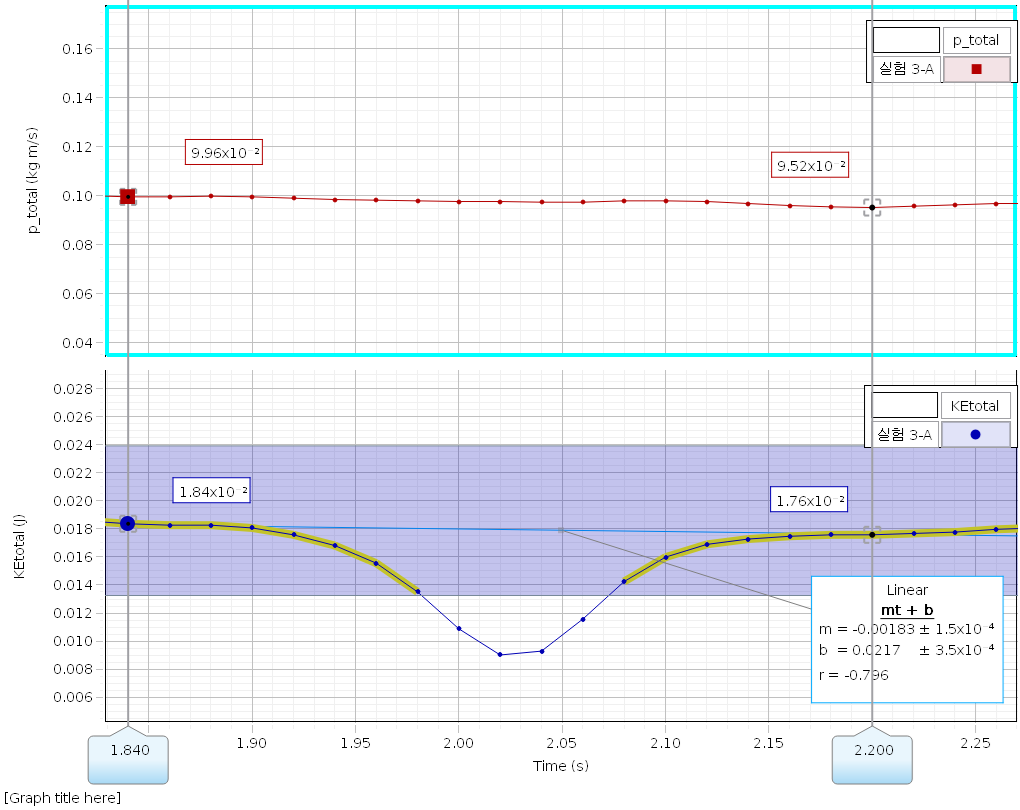
\includegraphics[height=4.36cm]{W10_elastic.png}
        \caption{\label{fig4-C}탄성 충돌}
    \end{subfigure}
    \caption{\label{fig4}}
\end{figure}
\clearpage
\section{실험 고찰}
\subsection{어떤 종류의 충돌에서 운동량이 보존되는가?}
Figure~\ref{table1}$\sim$Figure~\ref{fig4}의 그래프를 보면, 모든 종류의 충돌에서
항상 운동량을 보존됨을 알 수 있다.
\subsection{어떤 유형의 충돌에 대해 에너지가 보존되는가?}
Figure~\ref{table1}$\sim$Figure~\ref{fig4}의 그래프를 보면, 폭발하는 상황과 탄성
충돌하는 상황에서 에너지가 보존된다는 것을 알 수 있다. 다만, 롼전 비탄성 충돌시엔
에너지가 보존되지 않는데, 이 때는 열 에너지나 소리 등으로 에너지가 소비된 것으로, 총
에너지는 소비된다.
\subsection{총속도는 충돌 전후에 보존되는가?}
Figure~\ref{table1}$\sim$Figure~\ref{fig4}의 그래프를 보면, 완전 비탄성 충돌
시에는 총속도가 보존되지는 않음을 알 수 있다. 그 이유는 두 물체가 딱 붙어서 한
물체처럼 움직이기 때문에 질량이 커짐에 따라 속도가 $\vec{P}=m\vec{v}$식에 따라
줄어들기 때문이다.
\subsection{폭발에서 얻어진 추가적인 운동 에너지는 어디에서 왔는가?}
카트에 있던 용수철의 위치 에너지가 폭발적으로 운동에너지로 전환된 것이다. 운동에너지는
용수철에서 왔다고 할 수 있다.
\subsection{충돌로 손실된 초기 운동 에너지는 어디로 간 것일까?}
충돌로 손실된 초기 운동에너지는 열에너지, 소리등으로 변환된 것이다.
\subsection{오차원인}
\begin{itemize}
    \item 카트 센서의 부정확함이 있는 것 같다. 왜냐하면 파란 카트에서는 초기 1$\sim$
        10번째 데이터에서 속도 데이터가 0으로 일정한데 빨간 카트에서는 그렇지 않기
        때문이다.
    \item Figure\ref{fig2}를 보면, 이론값과의 차이가 조금 있음을 알 수 있는데,
        이는 이론상 마찰이나 공기 저항이 전혀 없기 때문으로, 실제 카트는 현실에서
        공기저항과 마찰 모두 있기 때문에 발생하는 오차이다. 이 경우, 벨크로 사이에서
        일정량의 에너지가 열이나 소리 에너지로 변환된 것임을 알 수 있다.
\end{itemize}
\subsection{오차를 줄이는 방법}
\begin{itemize}
    \item 카트 센서의 값을 확인하고 그 오차가 $\pm$몇 정도 되는지 확인하고
        그 값으로 보정하여 카트의 정확도를 올린다.
    \item 용수철의 핀을 건들 때엔 손이 아닌 도구를 사용하여 눌러서 손의 떨림을 카트에
        전달하지 않도록 한다.
\end{itemize}
\subsection{실험원리의 실생활에서의 예}
\begin{itemize}
    \item 당구를 칠 때의 당구공의 움직임
    \item 볼링을 칠 때의 볼링공의 움직임
\end{itemize}
\end{document}